\documentclass{article}
\usepackage{naturetex}

\renewcommand{\baselinestretch}{1.5}

\begin{document}

\maketitle

{\setstretch{1.0}
	% *** ABSTRACT ***
	\section*{Abstract}
	\lipsum[1]
}% setstretch

% *** INTRO ***
\newpage
\section*{Introduction}
\lipsum[2][1-4]
\cite{koch2015siamese}
\lipsum[2][5-100]

% *** RESULTS ***
\newpage
\section*{Results}\label{results}
\subsection*{\lipsum[10][1]}

\lipsum[3][1-4]
\cite{pearson1901liii}
\lipsum[3][5]
(\ref{fig:my_plot1})
\lipsum[3][6]
(\ref{sup.fig:my_sup_plot1})
\lipsum[3][7-100]

\begin{figure}[h]
	\begin{center}
		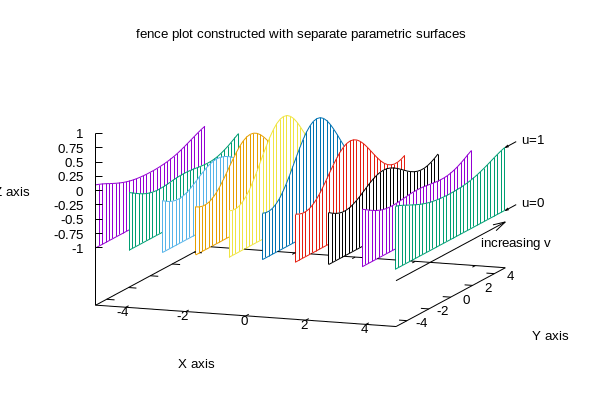
\includegraphics[width=0.75\textwidth]{fig1}
	\end{center}
	\caption{}
	\label{fig:my_plot1}
\end{figure}

% *** DISCUSSION ***
\newpage
\section*{Discussion}
\lipsum[4]

% *** METHODS ***
\newpage
\section*{Methods}
\subsection*{\lipsum[10][2]}
\lipsum[15]

\begin{figure}[h]
	\begin{center}
		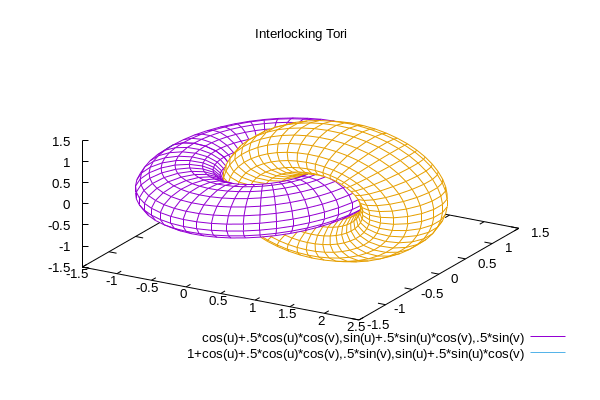
\includegraphics[width=0.75\textwidth]{fig2}
	\end{center}
	\caption{}
	\label{fig:my_plot2}
\end{figure}

\subsubsection*{\lipsum[10][3]}
\lipsum[13][1]
\cite{hinton2006reducing, chollet2015keras}
\lipsum[13][2-3]
\ref{fig:my_plot2}, \ref{sup.fig:my_sup_plot2}, and \ref{sup.fig:my_sup_plot3}.

\subsection*{Code availability}
\lipsum[5]

\subsection*{Data availability}
\lipsum[6]

% *** REFERENCES ***
\newpage
\bibliography{bibliography}
\bibliographystyle{naturemag}

% *** END NOTES ***
\newpage
\section*{End Notes}
\subsection*{Acknowledgements}
\lipsum[7]

\subsection*{Author Contributions}
\lipsum[8]

\subsection*{Declaration of Interests}
The authors declare no competing interests.

% *** FIGURE LEGENDS ***
\newpage
\section*{Figure Legends}
\begin{itemize}
	\item[] \ref{fig:my_plot1}: \textbf{\lipsum[20][1]} \textbf{(A)} \lipsum[12][1] \textbf{(B)} \lipsum[12][2] \textbf{(C)} \lipsum[12][3] \textbf{(D)} \lipsum[12][4] \textbf{(E)} \lipsum[12][5]
	\item[] \ref{fig:my_plot2}: \textbf{\lipsum[20][2]} \lipsum[13][1-4]
\end{itemize}

% *** TABLES ***
\newpage
\section*{Tables}
\lipsum[9][1-2]

\end{document}
